\documentclass[conference]{IEEEtran}
\IEEEoverridecommandlockouts

% Mantener tipografía Times tanto con pdfLaTeX como con XeLaTeX/Tectonic.
\usepackage{iftex}
\ifPDFTeX
  \usepackage[T1]{fontenc}
  \usepackage[utf8]{inputenc}
\else
  \usepackage{fontspec}
  \setmainfont{texgyretermes}[
    Extension=.otf, UprightFont=*-regular, BoldFont=*-bold,
    ItalicFont=*-italic, BoldItalicFont=*-bolditalic]
  \setmonofont{texgyrecursor}[
    Extension=.otf, UprightFont=*-regular, BoldFont=*-bold,
    ItalicFont=*-italic, BoldItalicFont=*-bolditalic]
\fi
\usepackage[spanish,es-tabla]{babel}

\usepackage{cite}
\usepackage{amsmath,amssymb,amsfonts}
\usepackage{algorithmic}
\usepackage{graphicx}
\usepackage{textcomp}
\usepackage{xcolor}
\def\BibTeX{{\rm B\kern-.05em{\sc i\kern-.025em b}\kern-.08em
    T\kern-.1667em\lower.7ex\hbox{E}\kern-.125emX}}
\begin{document}

\title{Predicción de resultados del fútbol uruguayo mediante métodos de aprendizaje supervisado}

\author{
\IEEEauthorblockN{Thiago Rivas}
\IEEEauthorblockA{C.I. 5.475.680-3 \\
\textit{Facultad de Ingeniería} \\
\textit{Universidad de la República}\\
Montevideo, Uruguay \\
email@fing.edu.uy}
\and
\IEEEauthorblockN{2\textsuperscript{nd} Nombre Apellido}
\IEEEauthorblockA{\textit{Facultad de Ingeniería} \\
\textit{Universidad de la República}\\
Montevideo, Uruguay \\
email@fing.edu.uy}
\and
\IEEEauthorblockN{3\textsuperscript{rd} Nombre Apellido}
\IEEEauthorblockA{\textit{Facultad de Ingeniería} \\
\textit{Universidad de la República}\\
Montevideo, Uruguay \\
email@fing.edu.uy}
}

\maketitle

% =========================================================
% PRESUPUESTO DE ESPACIO (formato IEEE, 2 columnas, 10pt)
% Referencia: ~500 palabras/columna de solo texto, ~1000 palabras/página.
% Límite duro: 5 páginas TOTALES, incluyendo 1 tabla y 3 figuras ya
% reservadas en el esqueleto (ocupan aprox. 1.5 páginas equivalentes
% entre las tres + la tabla). Presupuesto de TEXTO detallado por
% sección/subsección en cada % TODO más abajo.
%
% RESUMEN POR SECCIÓN (para chequeo rápido de avance):
%   Abstract .......................  100-150 palabras
%   Introducción ...................  250-300 palabras
%   Trabajo relacionado (opcional) .   80-120 palabras (o se omite)
%   Dataset y preprocesamiento .....  550-650 palabras (6 subsecciones)
%   Modelos .........................  400-450 palabras (+ 3 ecuaciones)
%   Experimentación .................  180-220 palabras (+ 2 figuras)
%   Resultados ......................  350-400 palabras (+ tabla + fig.)
%   Conclusiones ....................  150-180 palabras
%   Uso de IA .......................   50-70 palabras
%   -------------------------------------------------------
%   TOTAL TEXTO ..................... ~2100-2600 palabras
%   + 1-2 tablas, 3-4 figuras -> ocupan el resto hasta las 5 páginas.
%
% Si al ir escribiendo una sección se pasa del número, recortar AHÍ
% antes de seguir con la siguiente — es más fácil ajustar sobre la
% marcha que recortar 500 palabras de golpe al final.
% =========================================================

\begin{abstract}
Se estudia la predicción de victoria local, visitante o empate en el fútbol uruguayo mediante atributos históricos causales y validación temporal. Se conserva un conjunto común de 14.705 partidos hasta 2023 y se evalúan 472 de 2024--2025. Para Naive Bayes propio y de scikit-learn, la selección secuencial de suavizado y atributos produce modelos equivalentes de diez entradas. Ambos alcanzan accuracy 0,4788 y macro-F1 0,4454, frente a 0,4619 y 0,3564 del baseline de diez años. La mayor dificultad son los empates. Estos resultados consolidan únicamente NB y baseline; la evaluación final conjunta con árboles y Random Forest permanece pendiente.
% Pendiente compartido: revisar este resumen al incorporar los otros modelos.
\end{abstract}

\begin{IEEEkeywords}
aprendizaje supervisado, árboles de decisión, Naive Bayes, predicción deportiva, fútbol uruguayo
\end{IEEEkeywords}

% =========================================================
\section{Introducción}
La predicción de resultados del fútbol uruguayo se plantea como un problema de clasificación supervisada con tres clases: victoria local (L), victoria visitante (V) y empate (E). A partir de registros históricos de partidos, se busca construir atributos disponibles antes del encuentro y estimar su resultado. El desafío no consiste únicamente en ajustar un clasificador: también requiere respetar el orden temporal y evitar que el resultado que se intenta predecir intervenga en sus entradas.

En correspondencia con los objetivos de la tarea, el trabajo aborda la aplicación de herramientas metodológicas a datos reales, la implementación de métodos supervisados y el análisis de sus predicciones. Se implementaron un árbol ID3 con umbral mínimo de ganancia de información, un Naive Bayes categórico con suavizado mediante tamaño equivalente de muestra y el clasificador base de proporción de victorias en los diez años anteriores. El notebook incorpora además árboles de decisión y Random Forest de scikit-learn. La comparación incluye también Naive Bayes categórico de esa biblioteca.

El procesamiento parte de seis tasas históricas de victoria y reserva 2024--2025 para evaluación. Para ambos NB, la validación seleccionó diez atributos: esas tasas más puntos y diferencia de gol por partido de cada equipo en hasta cinco antecedentes. Se examinan métricas por clase además de la proporción global de aciertos.

La evaluación final consolidada en este documento corresponde a ambos NB y al baseline. La comparación final con árboles y Random Forest queda pendiente; sus experimentos de validación se conservan sin anticipar conclusiones sobre test.

% =========================================================
% Trabajo relacionado es opcional: incorporar solo referencias verificadas
% si aportan al análisis y caben dentro de las cinco páginas totales.
\section{Conjunto de datos y preprocesamiento}
\label{sec:preprocesamiento}
% Presupuesto: aproximadamente 550--650 palabras.

\subsection{Descripción del dataset}
Se utiliza el subconjunto de fútbol uruguayo de la colección de David Schoch\cite{b1}, suministrado en un ZIP con un único CSV. El archivo contiene 15.207 filas y 17 columnas; tras la política de exclusión quedan 15.177 partidos, desde el 5 de marzo de 1932 hasta el 30 de junio de 2025. Por tanto, 2025 no representa un año completo. Los campos centrales son fecha, equipos local y visitante, y goles registrados (\texttt{gh}, \texttt{ga}).

\subsection{Limpieza de datos}
La carga normaliza espacios y tipos y exige goles enteros no negativos. Elimina una repetición exacta. La auditoría identifica siete grupos ambiguos de fecha y par de equipos, incluyendo localías invertidas: se excluyen sus 16 registros completos, sin elegir un marcador. Además, se excluyen cinco filas de prórroga y ocho de penales; todas estas exclusiones se aplican antes de construir historiales. Se conserva un registro de motivos y líneas del CSV. Las 175 filas admitidas con advertencias de múltiples encuentros de un equipo en una fecha mantienen sus fechas originales; no se dispone de evidencia para corregirlas. La causalidad se entiende respecto de las fechas registradas.

\subsection{Construcción de la variable objetivo}
Se adopta el resultado reglamentario sobre registros \texttt{full\_time=F}: L si $gh>ga$, V si $gh<ga$ y E si son iguales. La etiqueta se denomina \texttt{winner}. El diccionario de la fuente incluye prórroga y penales en los goles\cite{b1}, pero no separa marcadores reglamentarios; las ocho filas P del archivo presentan goles iguales. Se excluyen E/P por incertidumbre, sin reconstruir goles ni imponer empates. Esto limita la cobertura del estudio. Los goles actuales y \texttt{full\_time} no son entradas de los clasificadores.

\subsection{Atributos derivados}
Se construyen seis tasas: proporción de victorias en los últimos cinco partidos de cada equipo, proporción de victorias de ambos dentro del año calendario, proporción histórica de victorias del local jugando como local y proporción de victorias de ese local frente al visitante con la misma localía. Si hay menos de cinco antecedentes se usan los disponibles; la referencia anual no corresponde necesariamente a una temporada deportiva.

El cálculo recorre fechas y obtiene los atributos de todos los encuentros de un día antes de actualizar cualquier historial de ese día. Así excluye resultados simultáneos y futuros. Cuando no hay antecedentes se asigna $0{,}5$: esto evita equiparar ausencia de historial con cero victorias, pero puede coincidir con una tasa observada y no constituye una categoría independiente. Nombres de equipos y mes no integran las seis entradas; los nombres sirven para enlazar historiales. Para NB se agregan cuatro entradas: puntos por partido y diferencia de gol por partido en hasta cinco antecedentes, para local y visitante. Los puntos son 3/1/0 y la diferencia es goles a favor menos goles en contra; sin antecedentes se asignan $4/3$ y 0. Estas diez entradas, seleccionadas por validación, no incluyen goles del partido a predecir.

\subsection{Discretización}
El discretizador común produce códigos enteros para los modelos propios. Para las tasas de los últimos cinco partidos se fijan cortes en $0{,}3$ y $0{,}6$: baja si $x<0{,}3$, media si $0{,}3\leq x<0{,}6$ y alta en otro caso. Las otras ocho entradas del NB final usan terciles aprendidos solo con entrenamiento y reutilizados en validación o evaluación. Los cortes repetidos se eliminan, por lo que pueden resultar menos de tres intervalos; los empates entre valores tampoco garantizan grupos de igual tamaño. No existe un intervalo exclusivo para ``sin historial''. Los valores numéricos no finitos se imputan con la mediana aprendida en entrenamiento.

\subsection{División temporal de datos}
Se reservan 14.705 partidos hasta 2023 para entrenamiento y 472 de 2024--2025 para evaluación. Los atributos de evaluación incorporan resultados de fechas anteriores del propio período, simulando predicciones sucesivas, sin reajustar el modelo. La misma política rige para el clasificador base: todos disponen de resultados de fechas anteriores, incluidos los del bloque de evaluación.

% =========================================================
\section{Modelos}
\label{sec:modelos}
% Presupuesto: aproximadamente 400--450 palabras, más tres ecuaciones.

\subsection{Clasificador base}
\texttt{TenYearWinRateClassifier} compara las tasas causales de victoria de los diez años anteriores, producidas por el mismo constructor de atributos. Incluye resultados de fechas anteriores del bloque evaluado y excluye el día actual. Sin antecedentes asigna $0{,}5$; ante igualdad elige al local. Nunca predice empate y no aprende parámetros ni modifica historiales al predecir.

\subsection{Árbol de decisión propio}
La implementación utilizada es \texttt{ID3}, en \texttt{src/id3.py}. En cada nodo selecciona el atributo de mayor ganancia de información y crea una rama por categoría observada. Para un conjunto $S$, con proporción $p_c$ de ejemplos de clase $c$, utiliza:
\begin{equation}
H(S) = -\sum_{c \in \{L,V,E\}} p_c \log_2 p_c
\label{eq:entropia}
\end{equation}
\begin{equation}
IG(S, A) = H(S) - \sum_{v \in valores(A)} \frac{|S_v|}{|S|} H(S_v)
\label{eq:ganancia}
\end{equation}
Los términos con $p_c=0$ se omiten. Cada atributo se usa como máximo una vez por rama. La recursión termina si el nodo es puro, no quedan atributos, se alcanza \texttt{max\_depth} (8 por defecto) o ninguna ganancia supera estrictamente \texttt{min\_info\_gain}. Este último criterio realiza prepoda. Cada nodo guarda su clase mayoritaria, que sirve de respaldo ante una categoría no observada; los empates se resuelven por orden de clase. El código contempla ramas vacías, aunque la construcción recorre únicamente categorías presentes.

\subsection{Naive Bayes propio}
\texttt{MEstimateCategoricalNB} estima las probabilidades de clase mediante frecuencias y supone independencia condicional entre atributos. Para el código $v$ del atributo $j$ y la clase $c$ aplica:
\begin{equation}
P(X_j=v\mid c)=\frac{n_{jvc}+m/K_j}{n_c+m}
\label{eq:m-estimate}
\end{equation}
Aquí $n_{jvc}$ cuenta coincidencias de código y clase, $n_c$ cuenta ejemplos de la clase y $K_j$ es el máximo código de entrenamiento más uno, o el mínimo declarado mediante \texttt{min\_categories} si es mayor. La grilla declara cuatro códigos en ambos NB, incluso con bines ausentes; en general $K_j$ puede variar entre atributos y un único $\alpha=m/K$ solo es equivalente con un dominio común de tamaño $K$. El cero queda reservado para desconocidos. El parámetro $m>0$ es el tamaño equivalente de muestra: reparte un peso total $m$ uniformemente entre las $K_j$ categorías, agregando $m/K_j$ a cada conteo. Se decide por $\arg\max_c[\log P(c)+\sum_j\log P(X_j=x_j\mid c)]$, con desempate E/L/V. Los códigos fuera del dominio se remiten al cero; el prior de clase $P(c)=n_c/N$ no se suaviza.

\subsection{Modelos de referencia (scikit-learn)}
Los dos árboles de scikit-learn usan entropía: uno recibe los códigos de ID3 y otro las tasas continuas. Random Forest conserva 300 árboles, tasas continuas, semilla 42 y ponderación de clases en cada muestra bootstrap (\texttt{balanced\_subsample}). \texttt{CategoricalNB} utiliza la misma discretización, con cuatro códigos por atributo incluyendo cero. Su estimador usa $(n_{jvc}+\alpha)/(n_c+K_j\alpha)$. Con $K_j=4$, $\alpha=m/4$, prior de clase empírico y las mismas entradas, coincide con NB propio. Se respeta el suavizado indicado, sin truncarlo, y se aprende el prior de clase de train. Los dos NB finales usan diez atributos; los árboles conservan su configuración.

% =========================================================
\section{Experimentación}
\label{sec:experimentacion}
% PRESUPUESTO DE LA SECCIÓN COMPLETA: 180-220 palabras de TEXTO.
% Ojo: las 2 figuras de abajo son las que más espacio real consumen
% de todo el paper (aprox. 1/3 de columna cada una, ~2/3 de página en
% total entre las dos). Si el espacio aprieta más adelante, esta es
% la sección donde conviene achicar las figuras (side-by-side en una
% sola figura con 2 subplots) antes que recortar Resultados.

\subsection{Selección temporal de hiperparámetros}
Se validó en los años completos 2021, 2022 y 2023, con entrenamiento expansivo anterior a cada año. Las fechas no se dividen entre conjuntos y cada combinación ajusta un pipeline nuevo por fold. La selección utiliza macro-F1 medio con igual peso por año. El error graficado es $1-\mathrm{accuracy}$; el error de entrenamiento es de resustitución y no interviene en la elección.

Se exploraron seis umbrales ID3 entre 0 y $0{,}05$, cinco valores de $m$ entre $0{,}1$ y 1000, cinco de $\alpha=m/4$ y doce combinaciones de profundidad (4, 8, sin límite) y hoja mínima (1, 5, 20, 50) del bosque. Este mantiene 300 árboles y semilla 42. Ante empate exacto se favorece menor umbral o suavizado; para el bosque, menor profundidad y mayor hoja.

ID3 seleccionó $0{,}005$ (macro-F1 $0{,}3818$); ambos NB seleccionaron el menor suavizado ($m=0{,}1$, $\alpha=0{,}025$), con macro-F1 $0{,}3635$. Sus métricas coinciden, como corresponde al suavizado equivalente con cuatro códigos. Random Forest alcanzó $0{,}4228$ con profundidad sin límite y hoja 20, frente a $0{,}3753$ con hoja 1. Se conservaron los dos árboles de referencia y el baseline. El notebook incluye todas las curvas y métricas por año. Estos hallazgos de selección no son una evaluación independiente. El reajuste y test de NB se presentan en la sección~\ref{sec:resultados}; los de árboles quedan pendientes.

\subsection{Comparación acotada de atributos}
Con hiperparámetros fijos se compararon siete variantes: actuales, adición de puntos, diferencia de gol, ambas, tasas históricas de empate y retiro separado de cada historial de localía. Los mismos folds seleccionaron puntos y goles para ID3 y ambos NB: macro-F1 $0{,}4002$ y $0{,}3858$, respectivamente, con menor accuracy que sus versiones iniciales. Random Forest conservó las seis tasas ($0{,}4228$). Restringir predicciones a L/V, manteniendo todas las verdades E/L/V, redujo macro-F1 en las 28 comparaciones, aunque a veces aumentó accuracy. Son resultados de selección: NB conserva $m=0{,}1$ y $\alpha=0{,}025$, sin volver a optimizarlos sobre diez atributos ni consultar test. El macro-F1 NB anual es $0{,}3736$, $0{,}4312$ y $0{,}3526$. Reutilizar folds para decisiones sucesivas puede introducir optimismo.

\begin{figure}[htbp]
\IfFileExists{results/validation/figures/id3.png}{%
\centerline{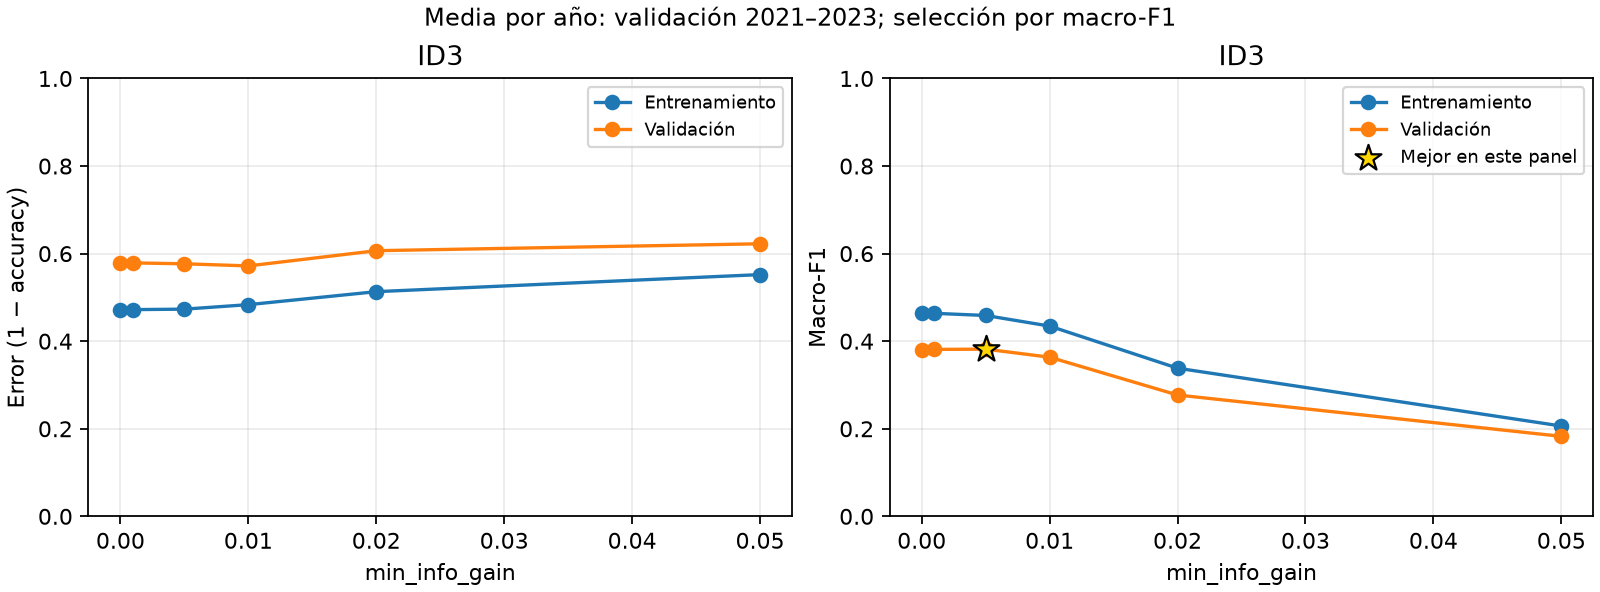
\includegraphics[width=0.9\linewidth]{results/validation/figures/id3.png}}
}{\centering\fbox{\parbox{0.85\linewidth}{\centering Figura pendiente de consolidación.}}}
\caption{Error y macro-F1 de entrenamiento/validación para ID3; medias de los tres años.}
\label{fig:hiperparam-arbol}
\end{figure}

\begin{figure}[htbp]
\IfFileExists{results/nb_delivery/figures/nb_error_report.png}{%
\centerline{\includegraphics[width=0.9\linewidth]{results/nb_delivery/figures/nb_error_report.png}}
}{\centering\fbox{\parbox{0.85\linewidth}{\centering Figura pendiente de consolidación.}}}
\caption{Error NB medio por año de validación, sobre las seis tasas iniciales. CategoricalNB coincide con $\alpha=m/4$. Se selecciona por macro-F1 antes de comparar atributos.}
\label{fig:hiperparam-nb}
\end{figure}

% =========================================================
\section{Resultados}
\label{sec:resultados}
% PRESUPUESTO DE LA SECCIÓN COMPLETA: 350-400 palabras de texto,
% sumado a la tabla y a la(s) figura(s) de matriz de confusión.
% Esta es la sección con más peso relativo del informe (el enunciado
% pide explícitamente el análisis de resultados) — si sobra espacio
% de otras secciones, se lo lleva esta.

Ambos NB se ajustaron una vez con los 14.705 partidos hasta 2023 y se evaluaron sobre los mismos 472 encuentros. Los discretizadores y clasificadores permanecen fijos durante test. Las métricas agrupan todo el bloque; macro-F1 pondera E/L/V por igual y se usa cero para divisiones indefinidas.

\begin{table}[htbp]
\caption{Evaluación común 2024--2025; pendientes sin resultado final}
\label{tab:resultados}
\centering
\begin{tabular}{lrr}
\hline
Modelo & Accuracy & Macro-F1 \\
\hline
Baseline (diez años) & 0,4619 & 0,3564 \\
Árbol propio & Pend. & Pend. \\
Naive Bayes propio & 0,4788 & 0,4454 \\
Random Forest & Pend. & Pend. \\
Naive Bayes (sklearn) & 0,4788 & 0,4454 \\
\hline
\end{tabular}
\end{table}

Los NB coinciden en las 472 predicciones, conteos y dominios. Sus puntajes logarítmicos difieren como máximo $5{,}33\,10^{-15}$, sin modificar el argmax. Aciertan 226 partidos frente a 218 del baseline: +1,69 puntos porcentuales de accuracy y +0,0889 de macro-F1. Corrigen 73 errores del baseline, pero pierden 65 de sus aciertos; ambos aciertan 153 y ambos fallan 181. No se evaluó significación estadística.

\begin{table}[htbp]
\caption{Métricas por clase. Ambos NB tienen idénticos valores}
\label{tab:clases}
\centering
\begin{tabular}{llrrrr}
\hline
Modelo & Clase & Precision & Recall & F1 & $n$ \\
\hline
NB (ambos) & E & 0,3537 & 0,2214 & 0,2723 & 131 \\
 & L & 0,5475 & 0,6368 & 0,5888 & 190 \\
 & V & 0,4497 & 0,5033 & 0,4750 & 151 \\
Baseline & E & 0,0000 & 0,0000 & 0,0000 & 131 \\
 & L & 0,5021 & 0,6368 & 0,5615 & 190 \\
 & V & 0,4199 & 0,6424 & 0,5079 & 151 \\
\hline
\end{tabular}
% Pendiente compartido: incorporar métricas por clase de árboles/bosque
% tras su evaluación; no completar con resultados de validación.
\end{table}

\subsection{Matrices de confusión}
Con filas reales y columnas predichas en orden E/L/V:
\[
C_{\mathrm{NB}}=
\begin{pmatrix}29&54&48\\24&121&45\\29&46&76\end{pmatrix},
\quad
C_{\mathrm{base}}=
\begin{pmatrix}0&66&65\\0&121&69\\0&54&97\end{pmatrix}.
\]
L presenta las mejores precision, recall y F1, seguida de V y E. De los 246 errores NB, 102 (41,46\%) son empates confundidos con victorias: E$\to$L es el error más frecuente (54), seguido de E$\to$V (48). Las confusiones L$\leftrightarrow$V suman 91 y los falsos empates, 53. NB reconoce 29 de 131 empates, mientras el baseline nunca predice E. Mantiene 121 aciertos locales, pero reduce de 97 a 76 los visitantes: mejora F1 en E y L y empeora en V.

\subsection{Análisis cualitativo}
Se ordenaron los partidos por fecha, local y visitante y se tomó el primero de cada par (resultado real, predicción NB), cubriendo nueve celdas de confusión. Es una selección reproducible e ilustrativa, no representativa de frecuencias. El 11/03/2024, Montevideo Wanderers--Deportivo Maldonado terminó 0--0: NB predijo E y el baseline L. El 17/02/2024, CA Fenix--Danubio terminó 1--2 y ambos predijeron V. Como error, el 07/04/2024, CA Cerro--Rampla Juniors Futbol Club terminó 3--0: NB predijo E y el baseline L. Los marcadores se recuperaron del ZIP limpio, sin usarlos como entradas.

Se dividió todo test por el signo de la diferencia de puntos por partido en hasta cinco antecedentes. Con ventaja local NB acierta 116/216 (53,70\%); con igualdad, 15/39 (38,46\%); con ventaja visitante, 95/217 (43,78\%). El baseline acierta 99, 21 y 98, respectivamente. Es un diagnóstico posterior, sin buscar umbrales. Una posible explicación es una señal útil de forma local, pero cambia también la composición E/L/V: 62/106/48, 9/15/15 y 60/69/88. No se aislaron estos efectos; el macro-F1 NB por grupo es 0,3788, 0,3737 y 0,3741.

La discretización pierde diferencias dentro de cada bin; los históricos resumen ventanas de distinta extensión y omiten sus denominadores. Una tasa 0,5 puede ser observada o neutra: no demuestra falta de historial. Tasas, puntos y goles resumen partidos superpuestos, lo que hace plausible información compartida; no se midió dependencia condicionada a la clase ni su efecto. Estas limitaciones no son causas demostradas de los errores.

% =========================================================
\section{Conclusiones}
Para NB se completó un flujo desde el ZIP original: limpieza, atributos causales, selección temporal, ajuste final y análisis. El m-estimate propio reproduce CategoricalNB bajo las condiciones explícitas de dominio y suavizado. La mejora frente al baseline es modesta en accuracy y mayor en macro-F1; no es uniforme entre clases, y los empates siguen siendo la principal dificultad.

Las observaciones describen una evaluación secuencial con 2025 incompleto, no una predicción simultánea de dos años ni evidencia causal. Ningún resultado de test modificó atributos, suavizado o decisiones. La comparación global entre algoritmos queda abierta hasta incorporar la evaluación final de árboles y Random Forest.
% Pendiente compartido: conclusiones conjuntas después de esa evaluación.

\section*{Uso de Inteligencia Artificial}
En la parte de NB se utilizó Codex para asistir en el análisis de resultados, su integración en notebook e informe y la ejecución de verificaciones. Esta descripción se limita al trabajo registrado en esta sesión. \textbf{Pendiente de completar por los integrantes:} autoría y correos, herramientas utilizadas personalmente, tareas asistidas y revisión o validación humana efectivamente realizada. No se dispone de esos datos para cerrar la declaración.
% No existe AI_USAGE.md: no citar una declaración personal inexistente.

\begin{thebibliography}{00}
\bibitem{b1} D. Schoch, ``football-data,'' GitHub repository. [Online]. Available: https://github.com/schochastics/football-data
% TODO: agregar referencias adicionales si se citan en Trabajo relacionado.
\end{thebibliography}

\end{document}
